
\documentclass{article}
\usepackage{graphicx} % Required for inserting images
\usepackage[spanish]{babel}
\usepackage{xcolor,colortbl}
\usepackage{graphicx}
\usepackage{amsmath}

\title{Informe de Práctica de Laboratorio III}
\author{José M. Díaz M. (25.682.785) \and Sergio José Noguera (30.572.211)}
\date{29 de julio de 2025}

\begin{document}

\maketitle



\section{Explique cómo se organiza la memoria cuando un sistema utiliza memory-mapped I/O. ¿En qué región de memoria se suelen mapear los dispositivos? ¿Qué implicaciones tiene para las instrucciones lw y sw?}


\quad

{Se dice que un sistema utiliza Memory-Mappede I/O cuando los dispositivos de entrada y/o salida (E/S) del hardware, se comunican con la CPU como si fueran ubicaciones de memoria. La principal característica de esta llamada memoria es el espacio de direcciones unificado donde tanto la memoria principal como los registros de los dispositivos de E/S comparten el mismo bus de direcciones. Esto quiere decir que a cada dispositivo E/S se le tiene asignado un rango específico de direcciones dentro del espacio de direcciones general del sistema.}

\quad

{Los dispositivos de E/S suelen mapearse en una región de memoria reservada y dedicada para ellos, que no se utiliza para la RAM principal. En arquitecturas de 32 bits como MIPS, esta región se encuentra comúnmente en la parte superior del espacio de direcciones, es decir, en direcciones de memoria altas.}

\quad

{Tanto lw como sw son instrucciones para cargar y almacenar palabras respectivamente, son lo más común para acceder a la memoria. Su implicación en la Memory-Mapped I/O es que se utilizan para interactuar con los dispositivos de E/S, y esto lo hacen de las siguientes formas:}

\quad

\textbf{•   } \underline{lw (load word):} { Cuando la CPU ejecuta una instrucción lw con una dirección que corresponde a un registro de un dispositivo de E/S mapeado en memoria, el procesador lee el valor de ese registro del dispositivo. Se puede decir que es como leer una ubicación de memoria normal, pero en realidad, se está obteniendo información de estado o datos de entrada del periférico.}

\quad

\textbf{•   } \underline{sw (store word):}{ De manera similar, cuando la CPU ejecuta una instrucción sw con una dirección que corresponde a un registro de un dispositivo de E/S, el procesador escribe el valor en ese registro del dispositivo. Esto permite al programa enviar comandos o datos de salida al periférico.}

\quad
\newpage





\section{¿Cuál es la principal diferencia entre memory-mapped I/O y la entrada/salida por puertos? ¿Qué ventajas y desventajas tiene cada enfoque? ¿Por qué MIPS32 utiliza principalmente memory-mapped I/O?}

\quad

\textbf{La principal diferencia entre Memory-Mapped I/O y la entrada/salida por puertos:}

\quad

\textbf{•   } \underline{Memory-Mapped I/O (MMIO):} {Tanto los dispositivos E/S, como sus registros de control y datos se mapean directamente en el espacio de direcciones que la memoria RAM. La CPU interactúa con los dispositivos utilizando las instrucciones lw y sw, para acceder fácilmente a la memoria, cabe aclarar que para CPU no hay distinción entre leer un byte de la RAM y leer un registro de estado.}

\quad

\textbf{•   } \underline{La entrada/salida por puertos:}{ Los dispositivos de E/S no se mapean directamente en el espacio, e n su lugar tienen un espacio de direcciones separado y dedicado para ellos, distinto del espacio de direcciones de la memoria RAM. La CPU para acceder a estos dispositivos utiliza instrucciones de E/S especiales y dedicadas que dirigen la operación a un espacio de direcciones de E/S separado del espacio de direcciones de la memoria principal. }

\quad


\quad

\textbf{Ventajas del Memory-Mapped I/O (MMIO):}

\quad

\textbf{1.   }{Simplifica el diseño del procesador y el conjunto de instrucciones del CPU haciendo que no se requiera de instrucciones especiales de E/S. Las mismas instrucciones lw y sw se usan para todo.}

\quad

\textbf{2.   }{Mayor flexibilidad de acceso, Al ser tratados como memoria, los dispositivos de E/S pueden ser accedidos con todas las modalidades de direccionamiento disponibles para la memoria (directo, indirecto, indexado, etc.). Esto facilita la programación de controladores de dispositivos.}

\quad

\textbf{3.   }{Ofrece mayor eficiencia potencial, ya que el acceso a E/S puede ser más rápido por utilizar los mismos mecanismos de bus y caché que la memoria.}

\quad

\textbf{4.   }{Tiene Integración con La Unidad de Gestión de Memoria, esta puede aplicar protección de memoria y mapeo de direcciones virtuales también a los dispositivos de E/S, mejorando la seguridad y la gestión de recursos.}

\quad

\textbf{5.   }{Menos pines de control: El bus de control puede ser más simple, ya que no necesita distinguir entre operaciones de memoria y E/S a nivel de señalización.}

\quad

\textbf{Desventajas del Memory-Mapped I/O (MMIO):}

\quad

\textbf{1.   }{Tiene un consumo mayor en la memoria RAM, esto debido a que los dispositivos de E/S ocupan parte del espacio de direcciones de la memoria principal, lo que reduce la cantidad de RAM disponible para el programa.}

\quad

\textbf{2.   }{Su Rendimiento variable, siendo que, si un dispositivo de E/S es muy lento, una operación de lectura/escritura a un registro mapeado en memoria puede afectar el rendimiento general}

\quad

\textbf{3.   }{Los accesos a registros de E/S casi siempre deben ser no-cacheables, es decir no se puede almacenar en el cache, esto para evitar problemas de coherencia.}

\quad

\textbf{Ventajas de la entrada/salida por puertos:}

\quad

\textbf{1.   }{Espacio de direcciones de E/S separado: Mantiene el espacio de direcciones de la memoria principal completamente disponible para la RAM, lo que es ventajoso en sistemas con espacio de direcciones limitado o cuando se desea maximizar la RAM utilizable.}

\quad

\textbf{2.   }{Al requerir instrucciones especiales, el acceso a los puertos de E/S puede ser más fácilmente restringido por el sistema operativo, ofreciendo una mejor seguridad. Un programa de usuario en modo protegido no puede usar directamente IN/OUT sin permiso.}

\quad

\textbf{3.   }{La distinción entre operaciones de memoria y E/S está explícita en el código, lo que puede mejorar la claridad a la hora de programar.}

\quad

\textbf{4.   }{En sistemas con muchos dispositivos, la decodificación de direcciones para puertos puede ser más simple y económica si se usa un bus de E/S más pequeño.}

\quad

\textbf{DesVentajas de la entrada/salida por puertos:}

\quad

\textbf{1.   }{Su conjunto de instrucciones es más complejo, ya que el CPU necesita instrucciones dedicadas para E/S (IN, OUT), lo que aumenta la complejidad del diseño del procesador.}

\quad

\textbf{2.   }{Las instrucciones de E/S suelen ser más limitadas y menos flexibles, en sus modos de direccionamiento y en los registros que pueden utilizar.}

\quad

\textbf{3.   }{Requiere señales de control adicionales en el bus para diferenciar entre accesos a memoria y accesos a puertos de E/S.}

\quad

\textbf{4.   }{Menor velocidad potencial, esto debido a que el bus de E/S puede ser más lento que el bus de memoria principal, y las instrucciones especiales pueden introducir latencia adicional.}

\quad

\textbf{Razon por la que MIPS utiliza principalmen-
te memory-mapped I/O:}

\quad

{La arquitectura RISC que utiliza MIPS, busca tener un conjunto de instrucciones pequeño, uniforme y fácil de decodificar para el procesador en este caso las ya mencionadas instrucciones lw y sw que al tratar la E/S de la llamada memoria, la CPU no necesita lógica de control separada para E/S. También Aprovecha muy bien de La Unidad de Gestión de Memoria y el sistema de memoria al mapear la E/S en memoria, ya que gestiona el acceso a los dispositivos de E/S con las mismas capacidades de protección de memoria y traducción de direcciones que se aplican a la RAM. En resumen, principalmente se usa debido a que ofrece una simplificada y fácil forma de generar código para operaciones de E/S.}

\quad
\newpage






\section{En un sistema con memory-mapped I/O: ¿Qué problemas pueden surgir si dos dispositivos usan direcciones solapadas? ¿Cómo se evita este conflicto?}


\quad

{En un sistema con Memory-Mapped I/O (E/S Mapeada en Memoria), los problemas pueden surgir cuando dos dispositivos intentan ocupar el mismo rango de direcciones de memoria, volviendo al sistema inestable o inoperable. Los Problemas se pueden definir como:}

\quad

\textbf{1.   } \underline{Problemas Comportamiento impredecible y corrupción de datos:}  {Estos poder surgir tanto en lectura como escritura, el lectura, Si la CPU intenta leer de una dirección que es compartida por dos dispositivos, no se sabe cuál de los dos dispositivos responderá o si ambos intentarán poner datos en el bus al mismo tiempo, resultando en una lectura errónea o datos corruptos yen escritura si la CPU intenta escribir en una dirección solapada, ambos dispositivos podrían intentar interpretar y responder a la escritura simultáneamente haciendo que el sistema falle.}

\quad

\textbf{2.   } \underline{2. Problemas Conflictivos de bus:}  {Cuando dos dispositivos intentan responder a la misma dirección al mismo tiempo, ambos podrían intentar colocar datos en el bus de datos o controlar las líneas de control, causar fallos en la comunicación.}

\quad

\textbf{3.   } \underline{Problemas de Inestabilidad del sistema y bloqueos: }  {Debido a la corrupción de datos y los conflictos de bus, el sistema operativo o las aplicaciones que intenten interactuar con estos dispositivos se encontrarán con valores incorrectos, respuestas inesperadas o simplemente no podrán comunicarse, lo que llevará a bloqueos del sistema, errores de hardware o reinicios inesperados.}

\quad


\textbf{4.   } \underline{Problemas de Imposibilidad de operar ambos dispositivos: }  {Es posible que ninguno de los dispositivos funcionen correctamente, o que solo uno funcionen de manera intermitente, ya que sus operaciones se interferiría mutuamente.}

\quad

\textbf{Para evitar conflictos se puede:}

\quad

\textbf{1.   } \underline{Asignación única:}  {En la fase de diseño del sistema, a cada dispositivo se le asigna un rango de direcciones único y no solapado dentro del espacio de direcciones de E/S. El decodificador de direcciones se diseña para reconocer únicamente su rango asignado.}

\quad

\textbf{2.   } \underline{Estándares de asignación de direcciones: }  {reservar las direcciones altas del espacio de 32 bits para E/S, y luego subdividir esa región cuidadosamente, y crear un mapa de memoria detallado y coherente que especifique qué rangos de direcciones están reservados para la RAM, qué rangos para la ROM y qué rangos para cada dispositivo de E/S específico (controlador de disco, controlador de red, temporizadores, etc.). Este mapa debe ser coherente en todo el sistema.}

\quad

\textbf{3.   } \underline{Los Sistema operativos adecuados:}  {Los sistemas operativos modernos como Linux o Windows tienen mecanismos para gestionar recursos de hardware. Utilizan información proporcionada por el BIOS/firmware o detectan el hardware para asignar dinámicamente o confirmar las direcciones de E/S. Intentarán evitar conflictos, pero un conflicto a nivel de hardware o firmware es difícil de solucionar por software una vez que se ha producido. En sistemas más complejos, existen mecanismos como Plug and Play (PnP) o PCI/PCIe que permiten a los dispositivos negociar sus asignaciones de direcciones con el sistema operativo al inicio, reduciendo la probabilidad de conflictos manuales.}

\quad
\newpage






\section{¿Por qué se considera que el memory-mapped I/O simplifica el diseño del conjunto de instrucciones de un procesador? ¿Qué tipo de instrucciones adicionales serían necesarias si se usara E/S por puertos?}

\quad

{El memory-mapped I/O simplifica significativamente el diseño del conjunto de instrucciones de un procesador por varias razones fundamentales:}

\quad

\textbf{1 -  } {\underline{Unificación del conjunto de instrucciones: }}

\quad

\textbf{    •} { Utiliza las mismas instrucciones para memoria y dispositivos de E/S.}

\textbf{    •} { Elimina la necesidad de instrucciones especiales como IN y OUT.}

\textbf{    •} { Reduce la complejidad del diseño del procesador al minimizar el número de instrucciones únicas necesarias.}

\quad

\textbf{2 -  } {\underline{Simplificación de la arquitectura: }}

\quad

\textbf{    •} { Requiere menos lógica interna en el CPU.}

\textbf{    •} { Reduce el tamaño físico del procesador.}

\textbf{    •} { Consume menos energía al tener menos componentes.}

\textbf{    •} { Facilita la implementación y verificación del diseño.}

\quad

\textbf{3 -  } {\underline{Flexibilidad operacional: }}

\quad

\textbf{    •} { Permite utilizar todos los modos de direccionamiento disponibles para memoria también con dispositivos de  E/S.}

\textbf{    •} { Facilita las operaciones aritméticas y lógicas directamente sobre datos de dispositivos de E/S.}

\textbf{    •} { Reduce el número de instrucciones necesarias para realizar operaciones complejas.}

\quad

\textbf{4 -  } {\underline{Ventajas prácticas: }}

\quad

\textbf{    •} { Mejora la velocidad de acceso a dispositivos de E/S al usar el mismo mecanismo que para memoria.}

\textbf{    •} { Simplifica significativamente la programación al eliminar la distinción entre operaciones de memoria y de E/S.}

\textbf{    •} { Reduce la complejidad del código fuente necesario para manejar dispositivos periféricos.}

\quad

\textbf{Instrucciones Adicionales Necesarias en E/S por Puertos: }

\quad

{En el sistema de E/S por puertos (I/O Mapped I/O), se requieren tipos específicos de instrucciones adicionales que no existen en el sistema de memory-mapped I/O:}

\quad

{\underline{Instrucciones Básicas de E/S: }}

\quad

\textbf{    •} { IN (Entrada): Para leer datos desde dispositivos de entrada hacia registros del procesador.}

\textbf{    •} { OUT (Salida): Para enviar datos desde registros del procesador hacia dispositivos de salida.}

\quad

{\underline{Variantes Específicas: }}

\quad

\textbf{    •} { INB/OUTB: Para operaciones de un byte.}

\textbf{    •} { INW/OUTW: Para operaciones de dos bytes (palabra).}

\textbf{    •} {INL/OUTL: Para operaciones de cuatro bytes (longitud).}

\quad

{Esta simplificación es especialmente importante en sistemas modernos donde la eficiencia y la simplicidad del diseño son fundamentales para el rendimiento general del sistema.}

\quad
\newpage






\section{¿Qué ocurre a nivel del bus de datos y direcciones cuando el procesador accede a una dirección de memoria que corresponde a un dispositivo? ¿Cómo sabe el hardware que debe acceder a un periférico en lugar de la RAM?}

\quad

{Cuando el procesador intenta acceder a una dirección de memoria que corresponde a un dispositivo, se produce una secuencia coordinada de eventos en los buses de datos y direcciones. El proceso funciona de la siguiente forma:}

\quad

\textbf{Secuencia de Eventos: }

\quad

\textbf{1)  } {El procesador genera una señal de dirección en el bus de direcciones.}

\textbf{2)  } {El dispositivo detecta su dirección específica en el bus de direcciones.}

\textbf{3)  } {El controlador del dispositivo responde mediante las líneas de control.}

\textbf{4)  } {Se establece la comunicación bidireccional a través del bus de datos.}

\quad

\begin{figure}[h]
    \centering
    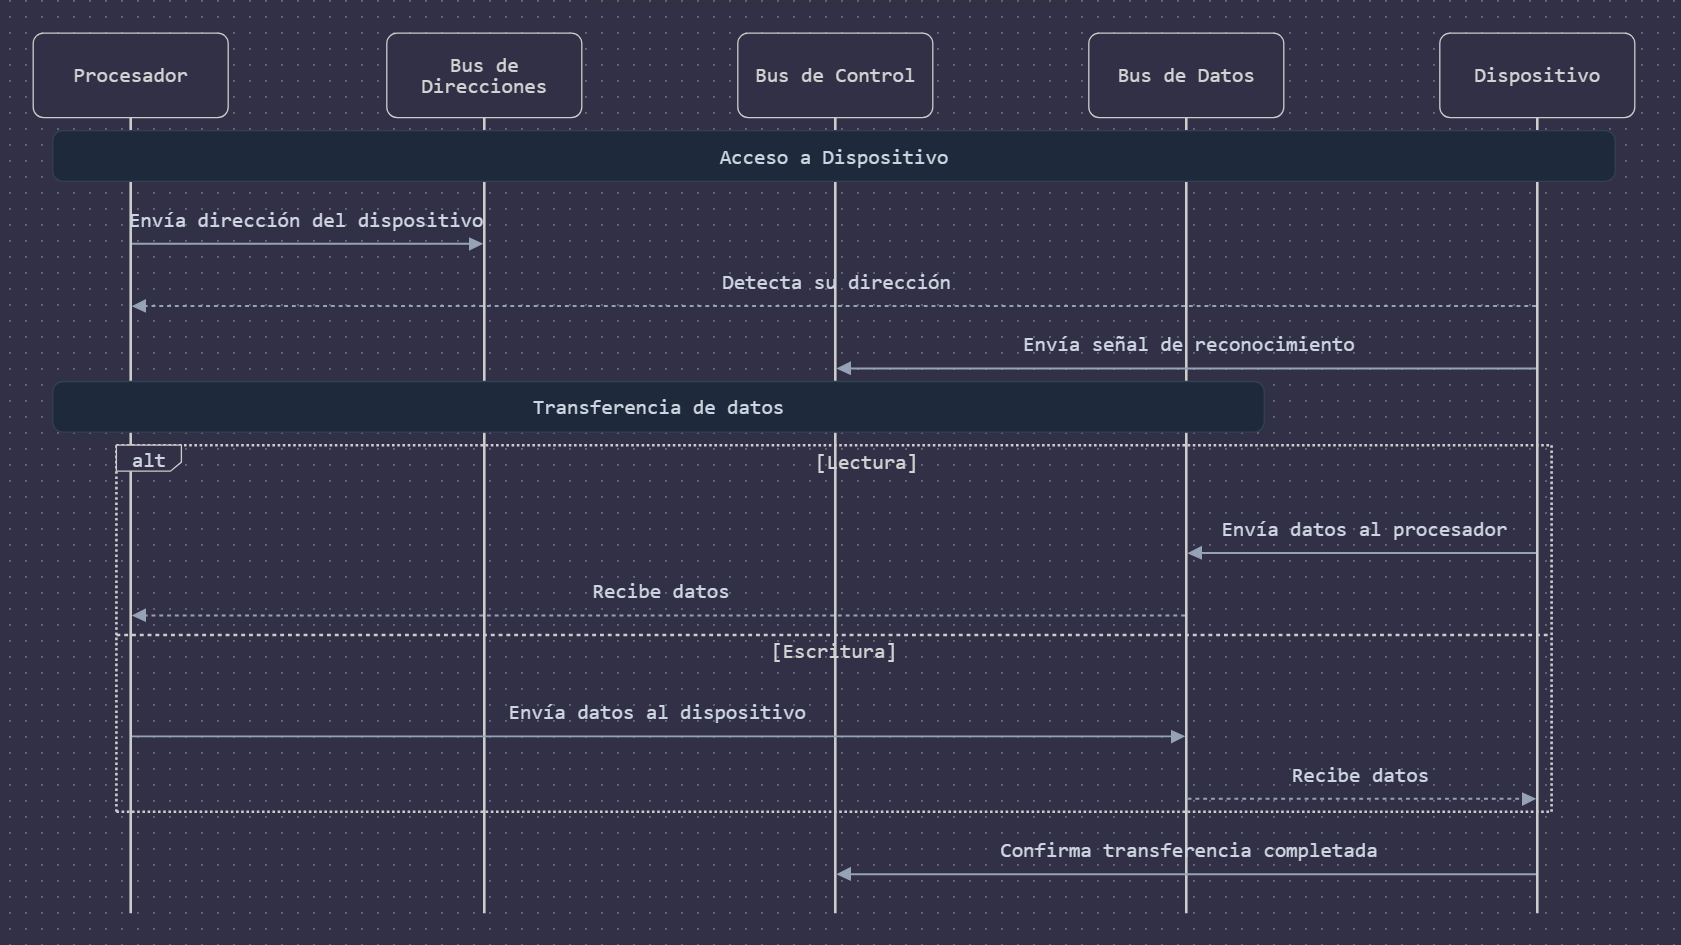
\includegraphics[width=10cm\textwidth]{figura_01.png}
    \caption{Procesador, Buses y Dispositivo}
    \label{fig:img1}
\end{figure}

{En la figura 1 se puede observar que:}

\quad

\textbf{    •} { Las flechas sólidas (→) representan señales activas enviadas por los componentes.}

\textbf{    •} { Las flechas punteadas (-->) indican respuestas o confirmaciones.}

\textbf{    •} { El bloque 'alt' muestra las dos posibilidades: lectura (el dispositivo envía datos) o escritura (el procesador envía datos).}

\quad

\textbf{Funcionamiento de los Buses: }

\quad

\textbf{1 -  } {\underline{Bus de Direcciones: }}

\quad

\textbf{    •} { Transmite la dirección específica del dispositivo.}

\textbf{    •} { Es independiente del bus de datos.}

\textbf{    •} { Los dispositivos monitorean constantemente este bus para detectar su dirección.}

\quad

\textbf{2 -  } {\underline{Bus de Control: }}

\quad

\textbf{    •} { Coordina el acceso entre todos los componentes.}

\textbf{    •} { Evita colisiones en la transferencia de datos.}

\textbf{    •} { Gestiona las señales de reconocimiento y confirmación.}

\quad

\textbf{3 -  } {\underline{Bus de Datos: }}

\quad

\textbf{    •} { Permite la transferencia bidireccional de información.}

\textbf{    •} { Se activa solo después de que el dispositivo reconoce su dirección.}

\textbf{    •} { La dirección de transferencia depende del tipo de operación (lectura o escritura).}



\quad

\textbf{Periférico en lugar de la RAM: }

\quad

{El hardware determina si debe acceder a un periférico o a la RAM mediante un mecanismo llamado "mapeo de memoria", que divide el espacio de direcciones en dos regiones distintas. El proceso funciona de la siguiente forma:}

\quad

\begin{figure}[h]
    \centering
    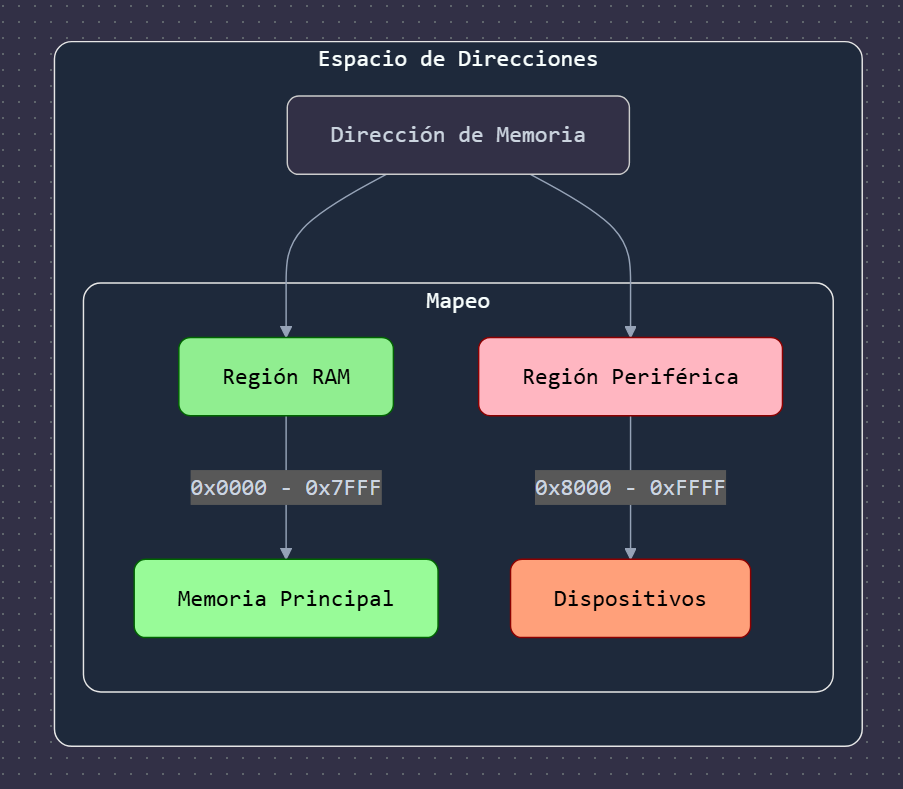
\includegraphics[width=5cm\textwidth]{figura_02.png}
    \caption{Mapeo de memoria}
    \label{fig:img2}
\end{figure}

\quad

{En la figura 2 se puede observar que:}

\quad

\textbf{    •} { Las direcciones más bajas (0x0000 - 0x7FFF) corresponden a la memoria RAM.}

\textbf{    •} { Las direcciones más altas (0x8000 - 0xFFFF) están reservadas para periféricos.}

\textbf{    •} { Esta división es estática y conocida por el hardware.}

\quad

\textbf{Mecanismo de Decisión: }

\quad

\textbf{1)  } {Cuando el procesador genera una dirección de memoria.}

\textbf{2)  } {El hardware verifica automáticamente si cae dentro del rango de RAM o periféricos.}

\textbf{3)  } {Basado en esta verificación, selecciona el camino apropiado.}

\quad

\textbf{Componentes Clave: }

\quad

\textbf{1 -  } {\underline{Decodificador de Direcciones: }}

\quad

\textbf{    •} { Hardware especializado que examina los bits más significativos de la dirección.}

\textbf{    •} { Actúa como un "conmutador" que dirige el acceso al destino correcto.}

\textbf{    •} { Funciona en nanosegundos para mantener el rendimiento del sistema.}

\quad

\textbf{2 -  } {\underline{Regiones de Memoria: }}

\quad

\textbf{    •} { RAM: Espacio para almacenar datos temporales y código en ejecución.}

\textbf{    •} { Periféricos: Puertos de entrada/salida, registros de control y buffers de dispositivos.}

\quad
\newpage






\section{¿Es posible que un programa normal (sin privilegios) acceda a un dispositivo mapeado en memoria? ¿Qué mecanismos de protección existen para evitar accesos no autorizados?}

\quad

{No, un programa normal sin privilegios no puede acceder directamente a un dispositivo mapeado en memoria. Este acceso está estrictamente controlado por el sistema operativo para garantizar la seguridad del sistema.}

\quad

\textbf{Razones técnicas: }

\quad

\textbf{1 -  } {\underline{Control de privilegios: }}

\quad

\textbf{    •} { Los dispositivos mapeados en memoria operan en modo kernel (privilegios elevados).}

\textbf{    •} { Los programas normales ejecutan en modo usuario (privilegios restringidos).}

\textbf{    •} { El sistema operativo implementa una barrera de seguridad entre estos modos.}

\quad

\textbf{2 -  } {\underline{Protecciones del sistema: }}

\quad

\textbf{    •} { La integridad de memoria protege el acceso a áreas sensibles.}

\textbf{    •} { El aislamiento del núcleo previene accesos no autorizados.}

\textbf{    •} { Las protecciones DMA (Acceso Directo a Memoria) evitan que dispositivos externos no autorizados accedan a la memoria del sistema.}



\quad

\textbf{Mecanismos de control: }

\quad

\textbf{1 -  } {\underline{Control de acceso: }}

\quad

\textbf{    •} { Los dispositivos tienen privilegios efectivamente iguales al nivel VTL0 (nivel de confianza más bajo, donde se ejecuta el sistema operativo tradicional y las aplicaciones en modo usuario y modo kerne).}

\textbf{    •} { Todo acceso DMA (Acceso Directo a Memoria) se marca con privilegios específicos.}

\textbf{    •} { El sistema operativo valida cada petición de acceso.}

\quad

\textbf{2 -  } {\underline{Capas de protección: }}

\quad

\textbf{    •} { Virtualización de hardware para aislar procesos críticos.}

\textbf{    •} { Verificación de código antes de su ejecución.}

\textbf{    •} { Monitoreo constante de accesos potencialmente peligrosos.}


\quad

\textbf{Acceso legítimo: }

\quad

{Para acceder a dispositivos mapeados en memoria, un programa debe:}

\quad

\textbf{1)  } {Ejecutarse con privilegios elevados.}

\textbf{2)  } {Utilizar APIs (Interfaces de Programación de Aplicaciones) del sistema operativo apropiadas.}

\textbf{3)  } {Obtener permisos específicos del sistema.}

\textbf{4)  } {Cumplir con las políticas de seguridad implementadas.}


\quad

\textbf{\underline{Mecanismos de Protección para Accesos no Autorizados: }}

\quad

 {Los sistemas modernos implementan múltiples capas de protección para prevenir accesos no autorizados a dispositivos mapeados en memoria. Estos mecanismos actúan en diferentes niveles, desde el hardware hasta el software, creando una defensa en profundidad contra amenazas potenciales.}



\quad

\textbf{Protecciones de Hardware: }

\quad

\textbf{1 -  } {\underline{IOMMU (Unidad de Gestión de Memoria de Entrada/Salida): }}

\quad

\textbf{    •} { Actúa como guardián principal del acceso a memoria.}

\textbf{    •} { Implementado como VT-d en Intel (Virtualización para E/S Dirigida) y AMD-Vi (AMD Virtualization: tecnología de virtualización desarrollada por AMD) en AMD (Advanced Micro Devices, Inc., es una empresa global de semiconductores).}

\textbf{    •} { Controla y valida todos los accesos DMA (Acceso Directo a Memoria) al espacio de direcciones físico.}


\quad

\textbf{2 -  } {\underline{Protección DMA  (Acceso Directo a Memoria) del Kernel: }}

\quad

\textbf{    •} { Previne accesos directos no autorizados a la memoria.}

\textbf{    •} { Especialmente importante para puertos PCI (Interconexión de Componentes Periféricos) y Thunderbolt.}

\textbf{    •} { Activa automáticamente cuando el equipo está bloqueado o cerrada la sesión.}



\quad

\textbf{Protecciones del Sistema Operativo: }

\quad

\textbf{1 -  } {\underline{Control de Memoria Virtual: }}

\quad

\textbf{    •} { El controlador de memoria virtual (MMU) gestiona el acceso a ubicaciones no autorizadas.}

\textbf{    •} { Implementa separación estricta entre espacio de usuario y kernel.}

\textbf{    •} { Valida cada petición de acceso a memoria.}


\quad

\textbf{2 -  } {\underline{Sistema de Controladores: }}

\quad

\textbf{    •} { Los controladores deben ser probados y firmados digitalmente.}

\textbf{    •} { Windows requiere firma digital de Microsoft para controladores.}

\textbf{    •} { Prevención de carga de controladores no confiables.}





\quad

\textbf{Protecciones Adicionales: }

\quad

\textbf{1 -  } {\underline{Integridad de Memoria: }}

\quad

\textbf{    •} { Crea un entorno aislado mediante virtualización de hardware.}

\textbf{    •} { Verifica el código antes de su ejecución.}

\textbf{    •} { Previne la manipulación por parte de programas malintencionados.}


\quad

\textbf{2 -  } {\underline{Aislamiento del Núcleo: }}

\quad

\textbf{    •} { Protege los procesos principales de Windows del software malintencionado.}

\textbf{    •} { Ejecuta procesos críticos en un entorno virtualizado.}

\textbf{    •} { Previne la explotación de vulnerabilidades.}




 
\quad

\textbf{Medidas de Prevención: }

\quad

\textbf{1 -  } {\underline{Seguridad Física: }}

\quad

\textbf{    •} { Protección contra dispositivos maliciosos conectados.}

\textbf{    •} { Desactivación de puertos no utilizados en BIOS/UEFI.}

\textbf{    •} { Control de acceso físico a los equipos.}


\quad

\textbf{2 -  } {\underline{Protección de Datos: }}

\quad

\textbf{    •} { Cifrado de datos sensibles en memoria.}

\textbf{    •} { No almacenar información confidencial sin cifrar en RAM.}

\textbf{    •} { Implementación de medidas de seguridad adicionales para datos criptográficos.}

\quad

{Estos mecanismos trabajan en conjunto para crear una barrera robusta contra accesos no autorizados, protegiendo tanto el hardware como el software del sistema. La combinación de protecciones de hardware y software proporciona una defensa en profundidad que hace extremadamente difícil para los atacantes obtener acceso no autorizado a dispositivos mapeados en memoria.}

\quad
\newpage





\section{¿Qué técnicas se pueden emplear para evitar esperas activas innecesarias al interactuar con dispositivos?}

\quad

{ La espera activa ocurre cuando un proceso consume recursos del CPU realizando verificaciones repetitivas sin realizar trabajo útil. Para evitar esperas activas innecesarias al interactuar con dispositivos, existen varias técnicas fundamentales que se pueden implementar. Las principales técnicas para optimizar estas interacciones: }

\quad

\textbf{1 -  } {\underline{Optimización de Eventos y Temporizadores: }}

\quad

\textbf{    •} { Evitar temporizadores recurrentes (setInterval: método que ejecuta repetidamente una función o un fragmento de código a intervalos regulares, especificados en milisegundos) que puedan interferir con interacciones del usuario.}

\textbf{    •} { Utilizar setTimeout (función que permite ejecutar un código o una función después de un período de tiempo especificado) de manera responsable, asegurándose de que las tareas no consuman demasiados recursos.}

\textbf{    •} { Implementar limpieza adecuada de temporizadores cuando ya no sean necesarios.}






\quad

\textbf{2 -  } {\underline{División de Tareas Costosas: }}

\quad

\textbf{    •} { Dividir operaciones pesadas en subtareas más pequeñas.}

\textbf{    •} { Permitir que el sistema procese otras interacciones entre fragmentos.}

\textbf{    •} { Utilizar scheduler.yield (método que permite a las aplicaciones web ceder el control del hilo principal del navegador, permitiendo que otras tareas de mayor prioridad se ejecuten) para permitir que el subproceso principal maneje otras tareas.}




\quad

\textbf{3 -  } {\underline{Gestión Eficiente de Recursos: }}

\quad

\textbf{    •} { Precargar datos anticipadamente cuando sea posible.}

\textbf{    •} { Implementar caché estratégicamente para reducir accesos a disco o red.}

\textbf{    •} { Minimizar operaciones de E/S durante interacciones críticas.}




\quad

\textbf{4 -  } {\underline{Optimización de Red y Conectividad: }}

\quad

\textbf{    •} { Agrupar transferencias de datos para minimizar el número de conexiones.}

\textbf{    •} { Reutilizar conexiones existentes en lugar de crear nuevas.}

\textbf{    •} { Implementar mecanismos de reintentos con backoff para fallos de red.}

\quad

{Al implementar estas técnicas de manera sistemática, es posible reducir significativamente las esperas activas innecesarias y proporcionar una experiencia más fluida y responsiva para los usuarios. La clave está en encontrar un equilibrio entre el rendimiento óptimo y el consumo eficiente de recursos del dispositivo.}

\quad
\newpage






\section{Análisis y Discusión de los Resultados}

{La mayor ventaja que tiene la Memory-Mapped I/O  sobre la entrada/salida por puertos, es su capacidad de simplificar conjuntos de instrucciones (no especiales) del procesador para que puedan tener fácil acceso a la memoria, su diseño como arquitectura RISC, busca la uniformidad y la eficiencia en el diseño del hardware del procesador y la facilidad de programación, puede que dependa completamente de la RAM pero esto trae más beneficio que problemas, solo se tiene que ser cuidado al asegurarse que cada dispositivo tenga un rango de direcciones de memoria único y exclusivo para su operación, y conocer las técnicas  para evitar esperas activas innecesarias al interactuar, como la optimización de eventos como la división de tareas costosas, la gestión eficiente de recursos y la optimización de red.}

\quad

{Una cosa a tomar muy en cuenta es que un programa sin privilegios no podrá acceder directamente a un dispositivo mapeado en memoria, debido a que el acceso está controlado por el sistema operativo que cuenta con sus mecanismos de protección como IOMMU y la gestión de memoria virtual para evitar accesos no autorizados, separando estrictamente el espacio de usuario y es sistema operativo que opera en modo kernel.}

\quad
\newpage


\end{document}
